\documentclass{beamer}
\usetheme{Madrid}
\usepackage[utf8]{inputenc}
\usepackage{graphicx}
\usepackage{listings}
\usepackage{xcolor}

\title[JackTrip Clients]{Modernizing JackTrip: Two New Hub Client Implementations}
\author{A.I. Assistant}
\institute{Networked Music Performance}
\date{\today}

% --- Custom Language Definitions for 'listings' ---
\definecolor{codegreen}{rgb}{0,0.6,0}
\definecolor{codegray}{rgb}{0.5,0.5,0.5}
\definecolor{codepurple}{rgb}{0.58,0,0.82}
\definecolor{backcolour}{rgb}{0.95,0.95,0.92}
\definecolor{keywordblue}{rgb}{0.13, 0.13, 1}

% Define a custom C++ language with specific keywords
\lstdefinelanguage{myC++}{
  morekeywords={void, const, QByteArray, QTcpSocket, QUdpSocket, QAudioSource,
            char, int, uint16_t, uint64_t, reinterpret_cast, static_cast,
            class, public, private, new, delete, if, else, for, while, return,
            qToLittleEndian, m_header, m_udpSocket, m_audioInputDevice, append},
  keywordstyle=\color{keywordblue}\bfseries,
  comment=[l]{//},
  commentstyle=\color{codegreen}\itshape,
  stringstyle=\color{codepurple},
  morestring=[b]",
  sensitive=true
}

% Define a custom JavaScript language with specific keywords
\lstdefinelanguage{myJS}{
  morekeywords={const, let, var, if, else, for, while, return, function, class,
            new, require, module, console, Buffer, WebSocket, Date, BigInt,
            on, alloc, writeUInt16LE, writeBigUInt64LE, copy, send, message},
  keywordstyle=\color{keywordblue}\bfseries,
  comment=[l]{//},
  commentstyle=\color{codegreen}\itshape,
  stringstyle=\color{codepurple},
  morestring=[b]',
  morestring=[b]",
  sensitive=true
}

% Define a global style for all listings
\lstdefinestyle{mystyle}{
    backgroundcolor=\color{backcolour},   
    numberstyle=\tiny\color{codegray},
    basicstyle=\scriptsize\ttfamily, % Font size reduced
    breakatwhitespace=false,         
    breaklines=true,                 
    captionpos=b,                    
    keepspaces=true,                 
    numbers=left,                    
    numbersep=5pt,                  
    showspaces=false,                
    showstringspaces=false,
    showtabs=false,                  
    tabsize=2,
    frame=single,
    framerule=0.5pt
}

\lstset{style=mystyle}

\begin{document}

\frame{\titlepage}

% --- Introduction to JackTrip ---
\begin{frame}
\frametitle{What is JackTrip?}
\begin{itemize}
    \item A system for high-quality, low-latency audio streaming over the internet.
    \item Designed specifically for networked music performance, enabling musicians to play together in real-time from different locations.
    \item Core technology relies on raw UDP packets for minimal overhead.
    \item Often used in a "Hub Server" model, where multiple clients connect to a central server that mixes and redistributes the audio.
\end{itemize}
\end{frame}

% --- The Challenge ---
\begin{frame}
\frametitle{The Challenge: Building Modern Clients}
The JackTrip hub server is a robust, command-line driven system. How can we build clients that are more accessible and integrate with modern platforms?
\vspace{1cm}
\begin{center}
    \large We will explore two distinct approaches:
    \begin{enumerate}
        \item A native desktop application using Qt6/C++.
        \item A web-based application using the Web Audio API and a proxy.
    \end{enumerate}
\end{center}
\end{frame}

% --- SLIDE 4: THE CORE PROMPTS (Final Version) ---
\begin{frame}[fragile]
  \frametitle{Core Prompts \& Citations}
  \scriptsize % Set default font size for the slide

  {\tiny\textbf{Prompt 1: Qt6/C++ Client}}
  \par
  You are a careful, concise assistant. Don't give commentary or anthropomorphize. Be very attentive to prompt continuations because they often create a single character syntax problem. The purpose is to make a qt6/c++ application that implements a JackTrip client that can connect to a running JackTrip hub server. It should connect with bi-directional audio and exchange JackTrip audio packets. Sample rate is 48000, bit depth is 16, channel count is 2, server IP address is 171.64.197.158. The initial handshake should initiate the connection on the canonical port and receive an ephemeral UDP port back from the server. This is described in the article uploaded. Also uploaded is an older working client but we want to modernize and use Qt6 audio.
  
  \par{\tiny\textbf{Prompt 2: Web App Conversion}}\par
  \textit{convert this working c++ project to a single-page web audio webapp using the most appropriate web udp streaming sockets}
  
  \par{\tiny\textbf{Prompt 3: WebRTC Postlude}}\par
  \textit{the presentation is ready, now the kicker, make a postlude in the presentation that accounts for the content of the webRTC article I've attached}
  
  \par{\tiny\textbf{Citations}}
  \setlength{\itemsep}{0pt} % Remove extra spacing between list items
  \begin{itemize}
      \item C. Chafe, "I am Streaming in a Room" Frontiers in Digital Humanities, vol. 5, 2018. \href{https://doi.org/10.3389/fdigh.2018.00027}{DOI: 10.3389/fdigh.2018.00027}
      
      \item \url{https://github.com/cchafe/hacktrip}: jacktrip hub client with rtaudio and library API.
      
      \item M. Sacchetto, P. Gastaldi, C. Chafe, C. Rottondi, and A. Servetti, “Web-Based Networked Music Performances via WebRTC: A Low-Latency PCM Audio Solution” J. Audio Eng. Soc., vol. 70, no. 11, pp. 926–937, (2022 November). \href{https://doi.org/10.17743/jaes.2022.0021}{DOI: 10.17743/jaes.2022.0021}
  \end{itemize}
\end{frame}

% --- Development Journey ---
\section{Development Journey}

\begin{frame}[fragile]
\frametitle{Development Journey: A Log of Prompts}
This project evolved through an iterative process of prompts and refinements:
\begin{itemize}\scriptsize
    \item \textbf{Initial Goal:} Create a Qt6/C++ JackTrip client.
    \item \textbf{Refinement:} Implement non-interleaved audio conversion.
    \item \textbf{Pivot:} Convert the C++ project to a single-page web audio app.
    \item \textbf{Debug 1:} Resolve "Unable to load a worklet's module" by embedding the script.
    \item \textbf{Debug 2:} Correct the TCP handshake byte order for the proxy.
    \item \textbf{Feature:} Add the required JackTrip header to audio packets in the proxy.
    \item \textbf{Debug 3:} Fix a `RangeError` by ensuring the sequence number wraps around.
    \item \textbf{Documentation:} Generate block diagrams (SVG, then PNG) and this LaTeX presentation.
    \item \textbf{Final Polish:} Refine LaTeX syntax highlighting and add the WebRTC postlude.
\end{itemize}
\end{frame}

% --- Implementation 1: Qt6/C++ ---
\section{Implementation 1: Native Qt6/C++ Client}

\begin{frame}
\frametitle{Architecture: Qt6/C++ Client}
This approach uses Qt's rich libraries to create a self-contained, high-performance native application.
\begin{figure}
    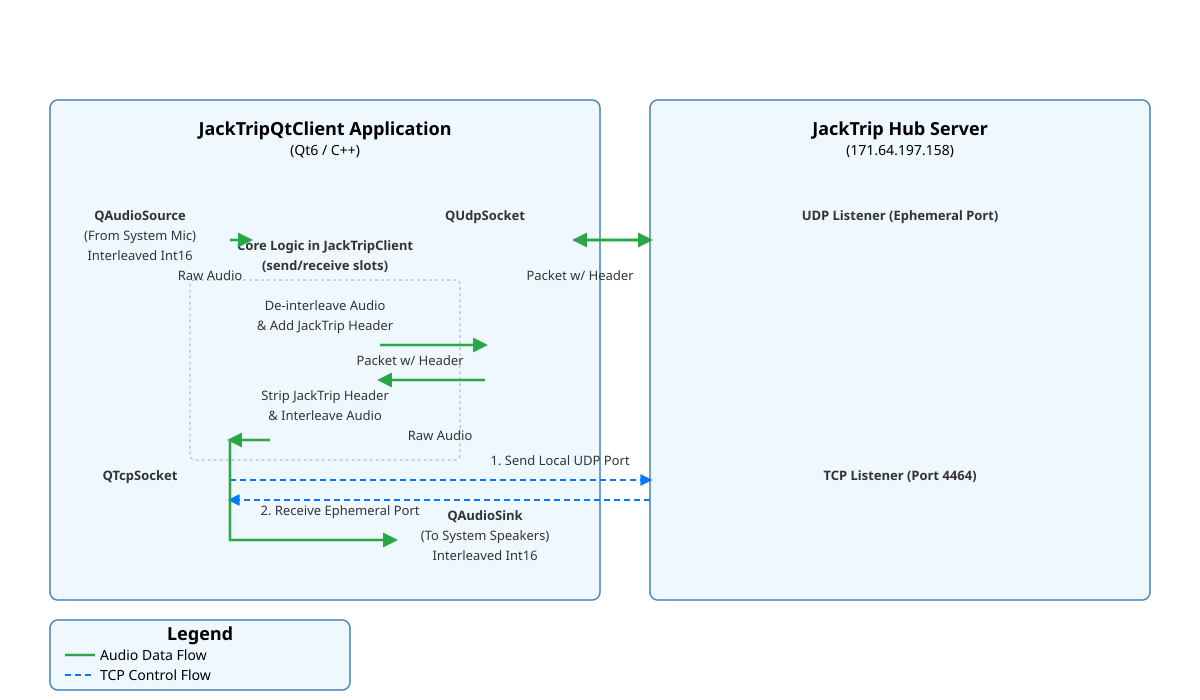
\includegraphics[width=1\textwidth]{qtTripDiagram.png}
    \caption{All logic is contained within a single application process.}
\end{figure}
\end{frame}

\begin{frame}[fragile]
\frametitle{Key Logic: Sending Audio Data}
The client performs two key steps before sending audio: de-interleaving the audio channels and prepending the JackTrip header.
\begin{lstlisting}[language=myC++]
void JackTripClient::sendAudioData()
{
    // 1. Read interleaved audio from QAudioSource
    QByteArray interleavedData = m_audioInputDevice->read(...);

    // 2. Convert to non-interleaved format for the server
    QByteArray nonInterleavedData(...);
    // ... de-interleaving logic ...

    // 3. Prepare and send packet with header
    QByteArray packet;
    m_header.SeqNumber = qToLittleEndian(m_sequenceNumber++);
    m_header.TimeStamp = qToLittleEndian(...);

    packet.append(reinterpret_cast<const char*>(&m_header), ...);
    packet.append(nonInterleavedData);
    
    m_udpSocket->writeDatagram(packet, ...);
}
\end{lstlisting}
\end{frame}

\begin{frame}
\frametitle{Qt6/C++ Client: Pros and Cons}
\begin{columns}[T]
    \begin{column}{0.5\textwidth}
        \textbf{Advantages}
        \begin{itemize}
            \item \alert<1>{High Performance}: Direct access to system resources and low-level networking.
            \item \alert<1>{Low Latency}: Minimal overhead between audio hardware and the network socket.
            \item \alert<1>{Self-Contained}: All logic in one executable.
        \end{itemize}
    \end{column}
    \begin{column}{0.5\textwidth}
        \textbf{Disadvantages}
        \begin{itemize}
            \item \alert<2>{Complex Deployment}: Requires compilation for each target platform (Windows, macOS, Linux).
            \item \alert<2>{Less Accessible}: Users must download and install a specific application.
            \item \alert<2>{Steeper Learning Curve}: Requires C++ and Qt knowledge.
        \end{itemize}
    \end{column}
\end{columns}
\end{frame}

% --- Implementation 2: Web Audio + Proxy ---
\section{Implementation 2: Web Audio + Proxy}

\begin{frame}
\frametitle{Architecture: Web Audio + Proxy}
This approach uses a standard web browser for the UI and a lightweight Node.js proxy to bridge the gap between web technologies and the JackTrip protocol.
\begin{figure}
    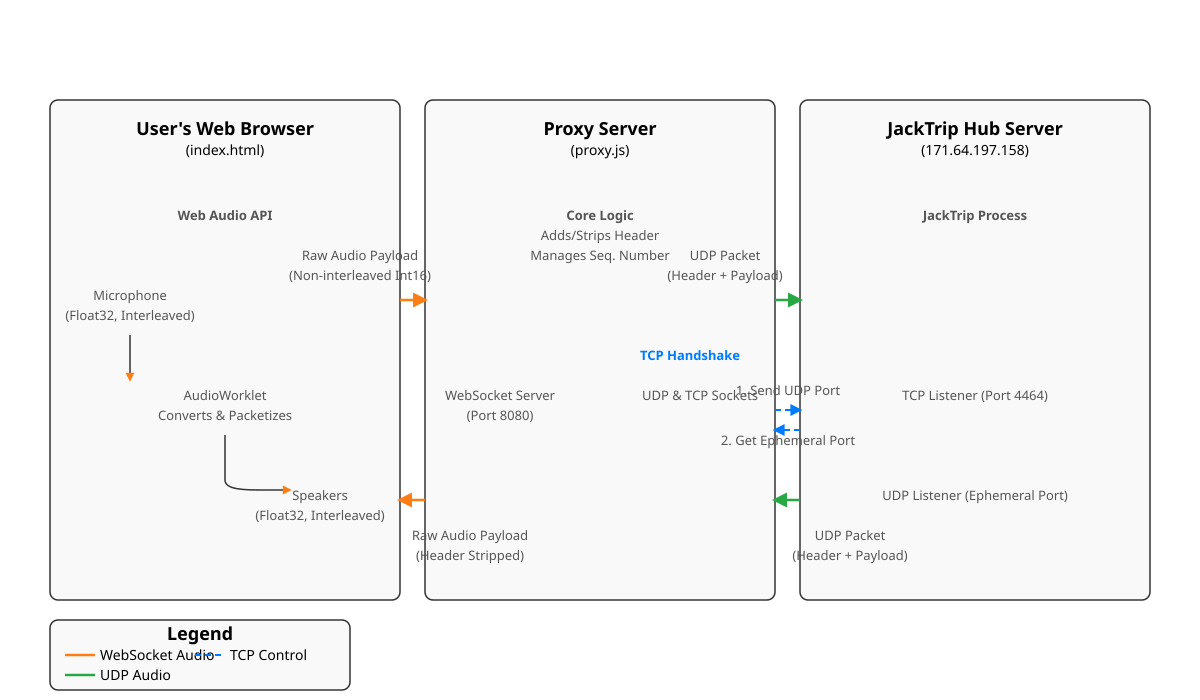
\includegraphics[width=1\textwidth]{webTripDiagram.png}
    \caption{A two-part system: the user-facing web app and the background proxy.}
\end{figure}
\end{frame}

\begin{frame}
\frametitle{The Proxy's Crucial Role}
\begin{itemize}
    \item Web browsers cannot create raw TCP or UDP sockets for security reasons.
    \item The proxy server acts as a translator:
    \begin{itemize}
        \item Speaks \alert<1>{WebSockets} to the browser.
        \item Speaks \alert<1>{raw UDP/TCP} to the JackTrip server.
    \end{itemize}
    \item It handles the entire JackTrip protocol, including the initial handshake and adding/stripping the header from every audio packet.
\end{itemize}
\end{frame}

\begin{frame}[fragile]
\frametitle{Key Logic: The Proxy Header}
The Node.js proxy adds the header before forwarding audio to the JackTrip server.
\begin{lstlisting}[language=myJS]
ws.on('message', audioPayload => {
    // Create a buffer for the full packet
    const packet = Buffer.alloc(HEADER_SIZE + audioPayload.length);

    // 1. Write the JackTrip header (all Little Endian)
    packet.writeBigUInt64LE(BigInt(Date.now()), 0);
    packet.writeUInt16LE(sequenceNumber, 8);
    // ... write other header fields ...

    // Increment and wrap the sequence number
    sequenceNumber = (sequenceNumber + 1) & 0xFFFF;

    // 2. Copy the audio payload from the web client
    audioPayload.copy(packet, HEADER_SIZE);

    // 3. Send the complete packet via UDP
    udpSocket.send(packet, ...);
});
\end{lstlisting}
\end{frame}

\begin{frame}
\frametitle{Web Audio Client: Pros and Cons}
\begin{columns}[T]
    \begin{column}{0.5\textwidth}
        \textbf{Advantages}
        \begin{itemize}
            \item \alert<1>{Maximum Accessibility}: Runs in any modern web browser. No installation needed.
            \item \alert<1>{Easy Deployment}: Simply host the HTML and JS files on a web server.
            \item \alert<1>{Rapid Development}: Faster UI development with web technologies.
        \end{itemize}
    \end{column}
    \begin{column}{0.5\textwidth}
        \textbf{Disadvantages}
        \begin{itemize}
            \item \alert<2>{Higher Latency}: Audio passes through more layers (Browser -> WebSocket -> Proxy -> UDP).
            \item \alert<2>{Complex Setup}: Requires a separate proxy server to be running.
            \item \alert<2>{Browser Limitations}: Dependent on Web Audio API performance and security policies.
        \end{itemize}
    \end{column}
\end{columns}
\end{frame}

% --- Comparison & Conclusion ---
\section{Conclusion}

\begin{frame}
\frametitle{Side-by-Side Comparison}
\begin{tabular}{l|l|l}
\hline
\textbf{Aspect} & \textbf{Qt6 / C++ Client} & \textbf{Web Audio + Proxy} \\
\hline
\hline
\textbf{Latency} & \alert<1>{Lowest} & Higher \\
\hline
\textbf{Accessibility} & Low (Requires install) & \alert<1>{Highest} (Browser-based) \\
\hline
\textbf{Deployment} & Per-platform binaries & Host web files, run proxy \\
\hline
\textbf{Complexity} & All in one app & Two-part system \\
\hline
\textbf{Best For} & Pro users, studios & Casual users, education \\
\hline
\end{tabular}
\end{frame}


\begin{frame}
\frametitle{Conclusion}
\begin{itemize}
    \item We have successfully implemented two modern clients for the classic JackTrip hub server.
    \item The \textbf{Qt6/C++} approach offers the highest performance and is ideal for professional, latency-critical applications.
    \item The \textbf{Web Audio} approach provides unparalleled accessibility and ease of use, opening up networked music performance to a much wider audience.
    \item Both models demonstrate the flexibility of the underlying JackTrip protocol and provide a path forward for its continued use and evolution.
\end{itemize}
\end{frame}

% --- POSTLUDE ---
\section*{Postlude: Future Work with WebRTC}

\begin{frame}
\frametitle{A More Direct Path: WebRTC}
The WebSocket+Proxy model works, but it has an inherent limitation: the proxy itself adds latency and is an extra point of failure.
\vspace{0.5cm}

\textbf{Question:} Can we connect the browser \textit{directly} to a JackTrip-like server?
\vspace{0.5cm}

\textbf{Answer:} Yes, by leveraging \alert{WebRTC}.
\vspace{0.5cm}

However, standard WebRTC (used for video calls) is unsuitable for music, as it applies audio compression and processing (echo cancellation, etc.) that distort the signal. The attached article provides a solution.
\end{frame}

\begin{frame}
\frametitle{The RTCDataChannel Solution}
The key insight from the research is to bypass WebRTC's media-processing pipeline and use the \textbf{RTCDataChannel}.
\begin{itemize}
    \item The `RTCDataChannel` is designed to send \alert<1>{arbitrary binary data}.
    \item This allows us to use the same architecture as our web client:
    \begin{itemize}
        \item Use `Web Audio` and an `AudioWorklet` to capture and packetize raw, non-interleaved audio.
        \item Send these raw packets directly over the `RTCDataChannel`.
    \end{itemize}
    \item This achieves a direct, low-latency connection from the browser to a server without unwanted audio processing.
\end{itemize}
\end{frame}

\begin{frame}
\frametitle{New Architecture: The Proxy-less Client}
This refined architecture eliminates the middleman, simplifying the system and reducing latency.
\begin{figure}
    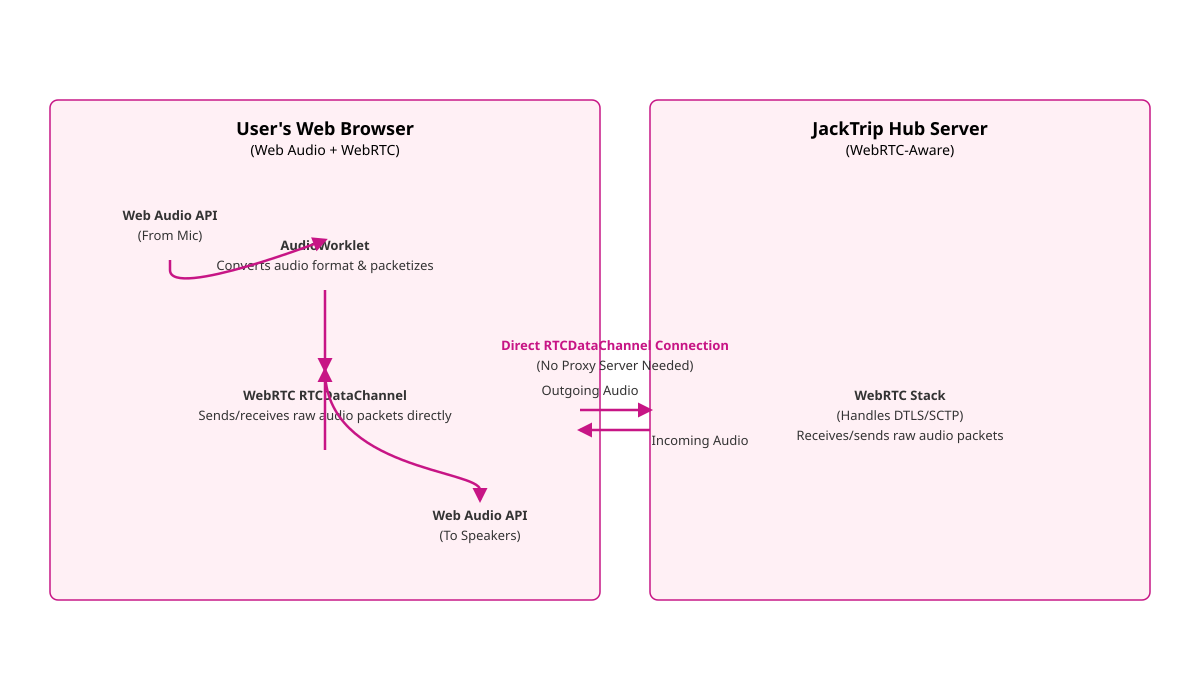
\includegraphics[width=1\textwidth]{webrtcTripDiagram.png}
    \caption{The browser connects directly to a WebRTC-aware server.}
\end{figure}
\end{frame}

\begin{frame}
\frametitle{The Future: WebRTC vs. WebSocket}
{\small % Start a group to apply small font size locally
\begin{tabular}{l|p{4.5cm}|p{4.5cm}}
\hline
\textbf{Aspect} & \textbf{WebSocket + Proxy (Current)} & \textbf{WebRTC DataChannel (Future)} \\
\hline
\hline
\textbf{Architecture} & 3-Tier (Browser-Proxy-Server) & \alert<1>{2-Tier (Browser-Server)} \\
\hline
\textbf{Latency} & Good, but with proxy overhead & \alert<1>{Potentially Lower} \\
\hline
\textbf{Server} & \textbf{Standard JackTrip Server} (via a required proxy) & \alert<2>{Must be modified} to be a WebRTC endpoint (handle DTLS/SCTP) \\
\hline
\textbf{Overall} & Highly accessible, proven to work & The ideal, most performant architecture for web-based clients \\
\hline
\end{tabular}
} % End the group
\end{frame}

\begin{frame}
\begin{center}
    \Huge Thank You
    \vspace{1cm}
    
    \Large Questions?
\end{center}
\end{frame}

\end{document}

